% Provenance (never printed): see sources/outline_sources.md (Year 3:
% speciation and saturation indices; carbonate equilibria applied to rocks;
% weathering kinetics; hydrothermal fluids). Brief: sources/book5/BRIEFS.md,
% ch. 15. Curves from figdata/bachelor-3/carbonate_system.py,
% activity_diagram.py, weathering_rates.py. Exercise and problem values in the
% Book 5 scratch calculator calc/ch15.py. The spring below the Varden
% limestone, its analysis and the granite stream are invented.
\chapter{Interacción agua--roca}\label{ch:b3:water-rock-interaction}

Un manantial al pie de un escarpe calizo deja una costra blanca en cada ramita
y piedra que toca; un arroyo que drena un granito transporta sílice, sodio y
un poco de potasio, y no deja costra alguna. La diferencia está en la química
del agua, y esa química es un registro de la roca que el agua atravesó: cuánto
dióxido de carbono transportaba, cuánto tiempo permaneció, qué minerales disolvió
y cuáles construyó. Este capítulo lee ese registro con las herramientas de la
química de disoluciones, desde el análisis de un agua hasta las velocidades de
disolución de los minerales y las trazas isotópicas de los fluidos calientes de la corteza.

\begin{recall}
Actividad, coeficiente de actividad, fuerza iónica, especiación, el producto de
solubilidad, alcalinidad, estado de saturación $\Omega$, ley de Henry, leyes de velocidad,
la ley de Arrhenius, estado de transición y valor $\delta$ se estudian en
los volúmenes universitarios de los libros de química. La meteorización química, la hidrólisis de
los silicatos, los minerales de la arcilla y la caolinita están en el volumen de primer año, en su
capítulo sobre meteorización y arcillas; la lisoclina y la profundidad de compensación de
los carbonatos, en su capítulo sobre sedimentos carbonatados, silíceos y evaporíticos. El fluido
hidrotermal aparece en el volumen de segundo año, en su capítulo sobre depósitos minerales, y
el termostato de meteorización de los silicatos en su capítulo sobre el clima a lo largo
del tiempo geológico; la circulación hidrotermal se trata en los libros escolares.
\end{recall}

\section{El análisis de un agua natural}\label{sec:b3:water-rock-interaction:analysis}

Un análisis de agua enumera los iones mayoritarios en miligramos por litro: calcio,
magnesio, sodio y potasio; bicarbonato, cloruro, sulfato y nitrato;
sílice disuelta como \ce{SiO2}; y el pH y la temperatura medidos en el
manantial, ya que ambos cambian una vez que la muestra sale de él. Al dividir
por la masa molar se obtienen milimoles por litro, y al multiplicar por la carga,
miliequivalentes. Un agua diluida es eléctricamente neutra, de modo que la suma de
los cationes debe igualar a la suma de los aniones.

\begin{method}[Comprobación de un análisis de agua]\label{met:b3:water-rock-interaction:analysis}
\begin{enumerate}
\item conviértase cada concentración a \unit{mmol/L} y a \unit{meq/L};
\item súmense los cationes y los aniones en \unit{meq/L};
\item calcúlese el error de balance de cargas $100\,(\sum\text{cat} -
  \sum\text{an})/(\sum\text{cat} + \sum\text{an})$, en por ciento;
\item acéptese el análisis si el error está dentro de 1 o \qty{2}{\percent} para
  un agua de 250 a \qty{1000}{mg/L}, algo más para una más diluida;
  en caso contrario, búsquese un ion ausente o un error analítico.
\end{enumerate}
\end{method}
% ledger: hem85:charge-balance

La actividad de un ion es su molalidad multiplicada por su coeficiente de
actividad $\gamma$. En aguas naturales $\gamma$ se calcula a partir de la fuerza iónica $I =
\tfrac12\sum m_i z_i^2$ con la ecuación extendida de Debye--Hückel
\[
-\log\gamma_i = \frac{A z_i^2\sqrt I}{1 + B a_i\sqrt I},
\]
con $A = 0.5085$ y $B = 0.3281$ para agua a \qty{25}{\celsius}, y un tamaño de
ion $a_i$ en ångströms: 9 para \ce{H+}, 8 para \ce{Mg^2+}, 6 para
\ce{Ca^2+}, 5 para \ce{CO3^2-}, 4 para \ce{Na+}, \ce{HCO3-} y \ce{SO4^2-},
3 para \ce{K+}, \ce{Cl-}, \ce{OH-} y \ce{NO3-}. La ecuación es válida hasta
unas \qty{0.1}{mol/L} de sales monovalentes, lo que cubre ríos y la mayoría de
las aguas subterráneas, pero no el agua de mar ni las salmueras. La temperatura
modifica $A$ solo entre 0.4883 a \qty{0}{\celsius} y 0.5425 a \qty{60}{\celsius},
de modo que los valores a \qty{25}{\celsius} sirven también para aguas frías.
% ledger: hem85:debye-huckel

El carbono inorgánico de un agua se reparte entre el dióxido de carbono disuelto
(escrito \ce{CO2} para la suma de \ce{CO2} y \ce{H2CO3}), el bicarbonato y el
carbonato, relacionados mediante
\[
K_1 = \frac{a_{\ce{HCO3-}}\,a_{\ce{H+}}}{a_{\ce{CO2}}}, \qquad
K_2 = \frac{a_{\ce{CO3^2-}}\,a_{\ce{H+}}}{a_{\ce{HCO3-}}}, \qquad
K_H = \frac{a_{\ce{CO2}}}{P_{\ce{CO2}}},
\]
con $\log K_1 = -6.35$, $\log K_2 = -10.33$ y $\log K_H = -1.47$ a
\qty{25}{\celsius}, y $-6.46$, $-10.49$ y $-1.27$ a \qty{10}{\celsius}
($P$ en atmósferas). Entre pH 6.4 y 10.3 domina el bicarbonato, y en la mayoría
de las aguas naturales la alcalinidad es casi toda bicarbonato. Un pH y un
bicarbonato medidos dan entonces las otras dos especies, y la presión parcial de
dióxido de carbono con la que el agua estaría en equilibrio.
% ledger: phreeqc:carbonate

\section{Saturación}\label{sec:b3:water-rock-interaction:saturation}

\begin{definition}[Índice de saturación]\label{def:b3:water-rock-interaction:si}
El \emph{índice de saturación (de un mineral)}\index{indice de saturación (de un mineral)@índice de saturación (de un mineral)}
en un agua es $\mathrm{SI} = \log(\mathrm{IAP}/K)$, donde IAP es
el producto de actividades iónicas del agua escrito como el producto de solubilidad
$K$ del mineral: $\mathrm{SI} = \log\Omega$.
\end{definition}

Un agua con $\mathrm{SI} < 0$ puede disolver el mineral, una con
$\mathrm{SI} > 0$ puede precipitarlo, y $\mathrm{SI} = 0$ corresponde al equilibrio.
Como la energía libre de la reacción de disolución es $\Delta_r G = RT\ln\Omega
= 2.303\,RT\,\mathrm{SI}$, el índice de saturación es también una medida de la
fuerza impulsora, en unidades de $2.303\,RT$, unos \qty{5.7}{kJ/mol} a
\qty{25}{\celsius}. Para la calcita $\mathrm{IAP} = a_{\ce{Ca^2+}}
a_{\ce{CO3^2-}}$ y $\log K = -8.45$ a \qty{25}{\celsius}, $-8.35$ a
\qty{10}{\celsius}: la calcita es más soluble en agua fría. Para el yeso, $\mathrm{SI} = \log(a_{\ce{Ca^2+}}a_{\ce{SO4^2-}}) + 4.55$;
para el cuarzo, cuya disolución da \ce{H4SiO4} neutro, $\mathrm{SI} = \log
a_{\ce{H4SiO4}} + 3.98$, y para la sílice amorfa la constante es 2.71
en lugar de 3.98. Los índices medidos llevan una incertidumbre de al menos $\pm0.1$,
y un agua dentro de $\pm0.3$ de cero se considera próxima al equilibrio.
% ledger: phreeqc:carbonate, phreeqc:silicates, hem85:si

\section{Equilibrios de carbonatos en las rocas}\label{sec:b3:water-rock-interaction:carbonate}

La calcita se disuelve en agua cargada de dióxido de carbono mediante
\[
\ce{CaCO3 + CO2 + H2O <=> Ca^2+ + 2 HCO3-},
\qquad K = \frac{a_{\ce{Ca^2+}}\,a_{\ce{HCO3-}}^2}{P_{\ce{CO2}}}
= \frac{K_{\mathrm{cal}}K_1K_H}{K_2},
\]
con $\log K = -5.94$ a \qty{25}{\celsius} y $-5.59$ a \qty{10}{\celsius}.
Cuánto se disuelve depende del origen del dióxido de carbono.

\begin{definition}[Sistemas carbonatados abiertos y cerrados]\label{def:b3:water-rock-interaction:open-closed}
Un agua disuelve la calcita en un \emph{sistema carbonatado abierto}\index{sistema carbonatado abierto}
cuando permanece en contacto con un gas de
$P_{\ce{CO2}}$ fija, que repone el dióxido de carbono consumido. Lo hace en un
\emph{sistema carbonatado cerrado}\index{sistema carbonatado cerrado} cuando antes se ha cargado de dióxido de carbono
y después queda aislada del gas, de modo que
el dióxido de carbono que contiene es todo el que puede utilizar.
\end{definition}

\begin{theorem}[Solubilidad de la calcita en sistemas abiertos y cerrados]\label{thm:b3:water-rock-interaction:calcite}
Para un agua de tipo bicarbonato cálcico, siendo $m$ la molalidad del calcio,
\[
\text{abierto:}\quad m = \left(\frac{K\,P_{\ce{CO2}}}{4\gamma_{\ce{Ca^2+}}
\gamma_{\ce{HCO3-}}^2}\right)^{1/3};
\qquad
\text{cerrado:}\quad 4\gamma_{\ce{Ca^2+}}\gamma_{\ce{HCO3-}}^2\,m^3 =
\frac{K_{\mathrm{cal}}K_1}{K_2}\,(C_0 - m),
\]
donde $C_0 = K_H P_{\ce{CO2}}$ es el dióxido de carbono captado antes de que el
sistema se cerrase.
\end{theorem}

\begin{proof}
Entre pH 6.5 y 8.5, el carbonato, \ce{H+} y \ce{OH-} son despreciables frente al
bicarbonato, así que el balance de cargas es $2m = m_{\ce{HCO3-}}$. Abierto: $K = \gamma
_{\ce{Ca^2+}}m\,\gamma_{\ce{HCO3-}}^2(2m)^2/P_{\ce{CO2}}$, lo que da la
raíz cúbica. Cerrado: cada calcio disuelto consume un \ce{CO2}, así que $m_{\ce{CO2}}
= C_0 - m$ y $a_{\ce{Ca^2+}}a_{\ce{HCO3-}}^2/a_{\ce{CO2}} = K/K_H =
K_{\mathrm{cal}}K_1/K_2$ da la cúbica.
\end{proof}

En el sistema abierto el calcio crece como la raíz cúbica de $P_{\ce{CO2}}$; en
el sistema cerrado está limitado por $C_0$, y el dióxido de carbono que queda al
final, así que la $P_{\ce{CO2}}$ final es mucho menor que la inicial. El
aire del suelo contiene de 10 a 100 veces el dióxido de carbono de la atmósfera, generado por las raíces
y por la descomposición de la materia vegetal, y las aguas subterráneas suelen mostrar
$P_{\ce{CO2}}$ entre $10^{-2.5}$ y $10^{-1}$ atmósferas. El agua en contacto
con calcita y aire contiene solo unos \qty{20}{mg/L} de calcio; la lluvia que
llega a una caliza atravesando un suelo, todavía abierta al gas del suelo, puede disolver
cuatro o cinco veces más. El karst se labra con este dióxido de carbono del suelo.
% ledger: hem85:pco2, phreeqc:carbonate

El camino de vuelta es la desgasificación. Un manantial que surge de una caliza transporta
la $P_{\ce{CO2}}$ del suelo y de la roca, de diez a cien veces la del
aire. Al aire libre pierde dióxido de carbono, el bicarbonato se convierte en
carbonato, el pH sube y el índice de saturación aumenta en más de una unidad,
como muestra el panel (b) de la figura siguiente para el manantial del
problema de fin de semana de este capítulo.
La calcita precipita en el lecho del arroyo y sobre musgos y ramitas: toba de
manantiales fríos, travertino de los cálidos. Los manantiales que atraviesan la roca
con rapidez, en días o semanas, por conductos, suelen llegar a la superficie
subsaturados; los que se filtran lentamente durante meses emergen cerca de
la saturación.
% ledger: hem85:pco2, usgsyvo:travertine

\begin{omfigure}
\begin{tikzpicture}
\begin{groupplot}[group style={group size=2 by 1, horizontal sep=1.6cm},
  omrecord, width=0.47\linewidth, height=0.42\linewidth, title style={font=\small},
  tick label style={font=\scriptsize}, label style={font=\small},
  legend style={font=\scriptsize, legend cell align=left}]
\nextgroupplot[title={(a) solubilidad de la calcita},
  xlabel={$\log P_{\ce{CO2}}$ (atm)}, ylabel={calcio disuelto (\unit{mmol/L})},
  xmin=-3.5, xmax=-1, ymin=0, ymax=5.5, clip=false,
  xtick={-3.5,-3,-2.5,-2,-1.5,-1}, xticklabels={$-3.5$,$-3$,$-2.5$,$-2$,$-1.5$,$-1$},
  legend style={at={(0.14,0.97)}, anchor=north west}]
\addplot[draw=none, fill=black!6, forget plot] coordinates {(-2.5,0) (-2.5,5.5) (-1,5.5) (-1,0)} -- cycle;
% computed in figdata/bachelor-3/carbonate_system.py
\addplot[omDef, thick] table[x=logp, y=ca_open10] {figdata/out/bachelor-3-carbonate_system-solubility.dat};
\addlegendentry{abierto, \qty{10}{\celsius}}
\addplot[red!70!black, thick] table[x=logp, y=ca_open25] {figdata/out/bachelor-3-carbonate_system-solubility.dat};
\addlegendentry{abierto, \qty{25}{\celsius}}
\addplot[omDef, thick, densely dashed] table[x=logp, y=ca_closed10] {figdata/out/bachelor-3-carbonate_system-solubility.dat};
\addlegendentry{cerrado, \qty{10}{\celsius}}
\addplot[red!70!black, thick, densely dashed] table[x=logp, y=ca_closed25] {figdata/out/bachelor-3-carbonate_system-solubility.dat};
\addlegendentry{cerrado, \qty{25}{\celsius}}
\draw[black, densely dotted] (axis cs:-3.37,0) -- (axis cs:-3.37,5.5);
\node[font=\scriptsize, anchor=south] at (axis cs:-3.37,5.5) {aire};
\node[font=\scriptsize, anchor=north, align=center] at (axis cs:-1.4,5.45) {aguas\\subterráneas};
\nextgroupplot[title={(b) desgasificación del manantial},
  xlabel={$\log P_{\ce{CO2}}$ (atm)}, ylabel={índice de saturación de la calcita},
  xmin=-3.5, xmax=-1.5, ymin=-0.2, ymax=1.9, x dir=reverse, clip=false,
  xtick={-3.5,-3,-2.5,-2,-1.5}, xticklabels={$-3.5$,$-3$,$-2.5$,$-2$,$-1.5$}]
% computed in figdata/bachelor-3/carbonate_system.py
\addplot[omDef, thick] table[x=logp, y=si] {figdata/out/bachelor-3-carbonate_system-degassing.dat};
\addplot[black, densely dotted, domain=-3.5:-1.5, samples=2] {0};
\addplot[red!70!black, only marks, mark=*, mark size=1.6pt] table[x=logp, y=si] {figdata/out/bachelor-3-carbonate_system-ends.dat};
\node[font=\scriptsize, anchor=north west] at (axis cs:-1.84,-0.01) {salida};
\node[font=\scriptsize, anchor=north west] at (axis cs:-3.3,1.55) {aire};
\end{groupplot}
\end{tikzpicture}

\par\smallskip{\small (a) Calcio disuelto por agua en equilibrio con
calcita, frente a la presión parcial de dióxido de carbono (para el sistema
cerrado, la presión a la que se cargó el agua): sistema abierto en trazo continuo,
sistema cerrado en trazo discontinuo; el agua fría disuelve más; la banda gris es el rango de
aguas subterráneas. (b) El manantial bajo la caliza de Varden, a \qty{10}{\celsius},
que pierde dióxido de carbono en su descenso por la ladera (leído de izquierda a derecha, en un eje invertido)
antes de que se forme calcita: su calcio y su alcalinidad quedan fijos, su pH sube
de 7.2 a 8.8, y su índice de saturación, de 0.04 a 1.6. Las constantes de equilibrio
proceden de una base de datos pública, y los coeficientes de actividad son los de
Debye--Hückel extendida.}\label{fig:b3:water-rock-interaction:calcite}
\end{omfigure}
% ledger: phreeqc:carbonate, hem85:debye-huckel, hem85:pco2, data:co2-mlo

La misma química, llevada a la escala del océano, se trata en los
volúmenes universitarios de los libros de química; la profundidad a la que el agua de mar
se vuelve subsaturada en calcita, la lisoclina, y la profundidad por debajo de la cual la calcita no
se acumula figuran en el volumen de primer año.

\begin{inthefield}[Un manantial que construye sus propias terrazas]
\begin{minipage}[t]{0.52\linewidth}\vspace{0pt}
En Palette Spring, uno de los Mammoth Hot Springs de la meseta de Yellowstone,
el agua termal asciende a través de una caliza enterrada y la transporta
disuelta. En superficie, el agua
se extiende sobre sus propios depósitos y pierde dióxido de carbono, y el carbonato cálcico
precipita como travertino, primero en el borde de cada poza, donde el agua es
más delgada. Los geólogos que estudian estos manantiales miden una sedimentación de unos
tres milímetros al día, quince veces el ritmo de las tobas calcáreas de los
manantiales fríos. Las franjas naranjas y
marrones son tapetes de microbios termófilos que viven en el agua de escorrentía caliente.
\end{minipage}\hfill
\begin{minipage}[t]{0.44\linewidth}\vspace{0pt}
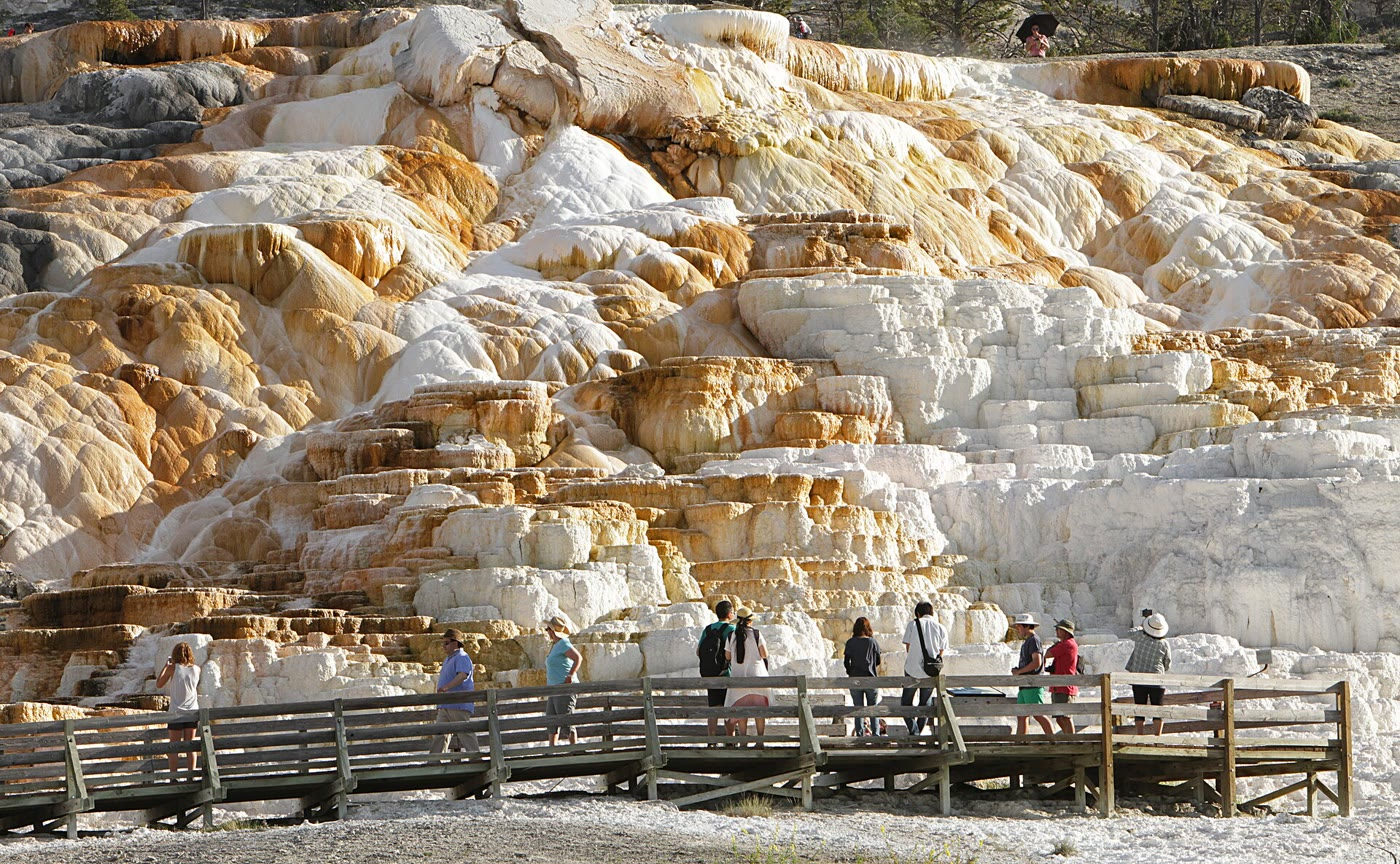
\includegraphics[width=\linewidth]{images/book5/b3-palette-spring-travertine.jpg}

{\scriptsize Terrazas de travertino de Palette Spring, Mammoth Hot Springs, con
una pasarela de madera y visitantes como escala. Fotografía de NPS por Jim Peaco, dominio público.}
\end{minipage}
\end{inthefield}
% ledger: photo:b3-palette-spring, usgsyvo:travertine, nps:travertine-terraces

\section{Cinética de la meteorización de silicatos}\label{sec:b3:water-rock-interaction:kinetics}

Los silicatos se disuelven mucho más lentamente que la calcita, y un agua rara vez alcanza
el equilibrio con ellos: su disolución debe describirse mediante una velocidad.

\begin{definition}[Ley de velocidad de disolución mineral]\label{def:b3:water-rock-interaction:rate-law}
La \emph{ley de velocidad de disolución mineral}\index{ley de velocidad de disolución mineral}
da la velocidad de disolución por unidad de superficie mineral, en
\unit{mol.m^{-2}.s^{-1}}, como suma de los mecanismos ácido, neutro y básico,
\[
r = \sum_j k_j\,e^{-\frac{E_j}{R}\left(\frac1T - \frac1{298.15}\right)}\,
a_{\ce{H+}}^{n_j}\,\bigl(1 - \Omega^{p_j}\bigr)^{q_j},
\]
con las constantes de velocidad $k_j$ a \qty{25}{\celsius}, las energías de activación $E_j$,
los órdenes de reacción $n_j$ (negativo para el mecanismo básico) y dos exponentes
$p_j$, $q_j$, que suelen tomarse como 1.
\end{definition}
% ledger: pk04:rate-law

\begin{proposition}[Lejos y cerca del equilibrio]\label{prop:b3:water-rock-interaction:affinity}
Con $p = q = 1$, la velocidad no depende de la saturación del agua
cuando $\Omega \ll 1$, y cerca del equilibrio es proporcional al
índice de saturación: $r \approx -2.303\,r_\infty\,\mathrm{SI}$, donde
$r_\infty$ es la velocidad lejos del equilibrio.
\end{proposition}

\begin{proof}
El factor es $1 - \Omega = 1 - 10^{\mathrm{SI}}$. Si $\mathrm{SI} \ll 0$, el factor
tiende a 1; para $\mathrm{SI}$ cercano a 0, $10^{\mathrm{SI}} \approx 1 +
2.303\,\mathrm{SI}$.
\end{proof}

Las constantes de velocidad proceden de experimentos de laboratorio con polvos minerales frescos,
en reactores de flujo mantenidos lejos del equilibrio. La figura siguiente dibuja
la ley de velocidad para cuatro minerales a \qty{25}{\celsius}. Cada curva tiene forma de V o de
U: los protones aceleran la disolución en agua ácida, el hidróxido en agua básica, y en
medio el mecanismo neutro fija un suelo. El olivino se disuelve unas tres
órdenes de magnitud más rápido que la albita a pH 5, por lo que es el primero
de los silicatos comunes en desaparecer de un suelo. Las energías de activación de
la albita y la forsterita, de 65 a \qty{79}{kJ/mol}, hacen que sus velocidades sean de cuatro a cinco
veces más rápidas a \qty{25}{\celsius} que a \qty{10}{\celsius}.
% ledger: pk04:rates

Las velocidades de campo son menores, en órdenes de magnitud. En experimentos en columna sobre un
granito recién triturado, la velocidad de la plagioclasa descendió de forma constante durante seis años
hasta \qty{7.0e-14}{mol.m^{-2}.s^{-1}}; el mismo granito, meteorizado de forma natural y
en parte transformado en caolinita, se disolvió a \qty{2.1e-15}{mol.m^{-2}.s^{-1}}
en las mismas condiciones, y ambas siguen siendo mucho más rápidas que la velocidad
medida en el propio perfil de meteorización. Para muchos minerales y edades, la
velocidad disminuye con el tiempo $t$ de meteorización del mineral según $R =
\num{3.1e-13}\,t^{-0.61}$ (mol\,m$^{-2}$\,s$^{-1}$, $t$ en años). Parte de
la caída se debe al mineral, cuyas superficies más reactivas se disuelven primero;
el resto se debe al entorno: agua lenta, mucho mineral para poco fluido, y
aguas intersticiales cercanas al equilibrio, donde la proposición anterior hace que la velocidad
sea pequeña.
% ledger: whitebrantley03:rates

\begin{omfigure}
\begin{tikzpicture}
\begin{axis}[omrecord, width=0.74\linewidth, height=0.46\linewidth,
  xlabel={pH}, ylabel={$\log r$ (\unit{mol.m^{-2}.s^{-1}})},
  xmin=0, xmax=14, ymin=-14.5, ymax=-6, clip=false,
  xtick={0,2,4,6,8,10,12,14}, ytick={-14,-12,-10,-8,-6},
  yticklabels={$-14$,$-12$,$-10$,$-8$,$-6$},
  tick label style={font=\scriptsize}, label style={font=\small},
  legend style={font=\scriptsize, legend cell align=left, at={(1.03,0.5)}, anchor=west}]
% computed in figdata/bachelor-3/weathering_rates.py
\addplot[green!45!black, thick] table[x=ph, y=forsterite] {figdata/out/bachelor-3-weathering_rates-curves.dat};
\addlegendentry{forsterita}
\addplot[omDef, thick] table[x=ph, y=albite] {figdata/out/bachelor-3-weathering_rates-curves.dat};
\addlegendentry{albita}
\addplot[red!70!black, thick, densely dashed] table[x=ph, y=kfeldspar] {figdata/out/bachelor-3-weathering_rates-curves.dat};
\addlegendentry{feldespato potásico}
\addplot[black, thick, densely dotted] table[x=ph, y=kaolinite] {figdata/out/bachelor-3-weathering_rates-curves.dat};
\addlegendentry{caolinita}
\end{axis}
\end{tikzpicture}

\par\smallskip{\small Velocidades de disolución lejos del equilibrio a
\qty{25}{\celsius}, frente al pH, a partir de una recopilación publicada de parámetros de
velocidad de laboratorio. El miembro final de la serie del olivino, la forsterita, no tiene mecanismo básico en
la recopilación; su curva deja de descender en el suelo neutro.}\label{fig:b3:water-rock-interaction:rates}
\end{omfigure}
% ledger: pk04:rates

\begin{definition}[Regímenes de meteorización]\label{def:b3:water-rock-interaction:regimes}
La meteorización química en un paisaje se halla en un \emph{régimen limitado
por el aporte}\index{régimen limitado por el aporte} cuando la limita la velocidad a la que
la erosión lleva minerales frescos al frente de meteorización, y en un
\emph{régimen limitado por la meteorización}\index{régimen limitado por la meteorización} cuando los minerales frescos
abundan y la velocidad de las reacciones lo limita.
\end{definition}

Una recopilación de pequeñas cuencas de drenaje muestra los dos casos. Donde la erosión es lenta, bajo
suelos espesos y lixiviados en relieves suaves, el flujo de meteorización sigue a la
velocidad de erosión: toda la roca fresca que llega queda totalmente lixiviada, y un clima más cálido o
más húmedo apenas lo modifica. Donde la erosión es rápida, en montañas escarpadas, el
flujo crece con la escorrentía, como la raíz cuadrada de la velocidad de erosión, y con
la temperatura, con una energía de activación aparente de $74 \pm
\qty{29}{kJ/mol}$. Solo en el segundo régimen puede la meteorización de silicatos actuar como
termostato climático del volumen de segundo año.
% ledger: west05:regimes

El mineral secundario que forma un agua de meteorización se lee en otro
diagrama.

\begin{definition}[Diagrama de actividad]\label{def:b3:water-rock-interaction:activity-diagram}
Un \emph{diagrama de actividad (estabilidad mineral)}\index{diagrama de actividad (estabilidad mineral)}
divide un plano de razones de actividad de un agua, como
$\log(a_{\ce{K+}}/a_{\ce{H+}})$ frente a $\log a_{\ce{H4SiO4}}$, en los
campos donde cada mineral de un sistema químico es el estable.
\end{definition}

\begin{proposition}[Fronteras de un diagrama de actividad]\label{prop:b3:water-rock-interaction:boundaries}
En el sistema \ce{K2O}--\ce{Al2O3}--\ce{SiO2}--\ce{H2O}, con el aluminio conservado en los sólidos
y el agua a actividad unitaria, un mineral con $k$ átomos de potasio, $a$ de aluminio y
$s$ de silicio por fórmula y constante de disolución $K$ (a \ce{K+},
\ce{Al^3+}, \ce{H4SiO4}) fija
\[
\log\frac{a_{\ce{Al^3+}}}{a_{\ce{H+}}^3} = \frac{\log K - kX - sY}{a},
\qquad X = \log\frac{a_{\ce{K+}}}{a_{\ce{H+}}},\quad Y = \log a_{\ce{H4SiO4}}.
\]
El mineral estable da la actividad de aluminio más baja, y la frontera
entre dos minerales es una recta en $(Y, X)$.
\end{proposition}

\begin{proof}
La disolución consume $h = k + 3a$ protones, por balance de cargas, de modo que $a\log
a_{\ce{Al^3+}} = \log K + h\log a_{\ce{H+}} - k\log a_{\ce{K+}} - s\log
a_{\ce{H4SiO4}}$; dividiendo por $a$ y pasando $3\log a_{\ce{H+}}$ a la izquierda
se obtiene la expresión. Un agua en equilibrio con un mineral está
subsaturada respecto de cualquier mineral que necesitara más aluminio, y
sobresaturada respecto de cualquiera que necesitara menos, así que el menos soluble es
el estable. Igualando dos de tales expresiones, lineales en $X$ y $Y$, se obtiene una recta.
\end{proof}

Con las constantes a \qty{25}{\celsius}, la gibbsita da paso a la caolinita en
$\log a_{\ce{H4SiO4}} = -4.39$ (\qty{2.4}{mg/L} de sílice) y la caolinita a
moscovita en $\log(a_{\ce{K+}}/a_{\ce{H+}}) = 1.55$, y el feldespato potásico es estable
solo en aguas ricas en potasio y sílice. El diagrama es la secuencia de meteorización
del volumen de primer año en cifras: un agua diluida que arrastra
el potasio y la sílice hace que un feldespato se transforme en gibbsita; un agua que
retiene más sílice forma caolinita; una que retiene más potasio, como en profundidad,
forma una mica.
% ledger: phreeqc:silicates

\begin{omfigure}
\begin{tikzpicture}
\begin{axis}[omrecord, width=0.66\linewidth, height=0.5\linewidth,
  xlabel={$\log a_{\ce{H4SiO4}}$}, ylabel={$\log(a_{\ce{K+}}/a_{\ce{H+}})$},
  xmin=-6, xmax=-2, ymin=0, ymax=10, clip=false,
  xtick={-6,-5,-4,-3,-2}, xticklabels={$-6$,$-5$,$-4$,$-3$,$-2$},
  tick label style={font=\scriptsize}, label style={font=\small}]
% computed in figdata/bachelor-3/activity_diagram.py
\addplot[black, thick, unbounded coords=jump] table[x=y, y=x] {figdata/out/bachelor-3-activity_diagram-lines.dat};
\addplot[omDef, densely dashed] table[x=y, y=x] {figdata/out/bachelor-3-activity_diagram-quartz.dat};
\addplot[omDef, densely dotted] table[x=y, y=x] {figdata/out/bachelor-3-activity_diagram-amorph.dat};
\addplot[red!70!black, only marks, mark=*, mark size=1.8pt] table[x=y, y=x] {figdata/out/bachelor-3-activity_diagram-samples.dat};
\node[font=\small] at (axis cs:-5.4,0.8) {gibbsita};
\node[font=\small] at (axis cs:-3.25,0.75) {caolinita};
\node[font=\small] at (axis cs:-4.6,5.0) {moscovita};
\node[font=\small] at (axis cs:-3.3,9.3) {feldespato potásico};
\node[font=\scriptsize, omDef, anchor=south] at (axis cs:-3.98,10) {cuarzo};
\node[font=\scriptsize, omDef, anchor=south] at (axis cs:-2.71,10) {sílice amorfa};
\node[font=\scriptsize, red!70!black, anchor=west] at (axis cs:-4.58,0.38) {A};
\node[font=\scriptsize, red!70!black, anchor=west] at (axis cs:-3.80,1.29) {B};
\node[font=\scriptsize, red!70!black, anchor=west] at (axis cs:-3.48,4.08) {C};
\end{axis}
\end{tikzpicture}

\par\smallskip{\small Campos de estabilidad en el sistema
\ce{K2O}--\ce{Al2O3}--\ce{SiO2}--\ce{H2O} a \qty{25}{\celsius}, con la saturación de cuarzo
(de trazos) y sílice amorfa (de puntos). Tres aguas inventadas: A, un arroyo diluido
tropical; B, un arroyo sobre granito; C, un agua subterránea profunda en
granito.}\label{fig:b3:water-rock-interaction:activity}
\end{omfigure}
% ledger: phreeqc:silicates

\section{Fluidos hidrotermales}\label{sec:b3:water-rock-interaction:hydrothermal}

El agua caliente que circula por la corteza, cerca de una dorsal o de una intrusión,
intercambia oxígeno con la roca que atraviesa. A alta temperatura el
fraccionamiento entre roca y agua es pequeño, y ambos tienden hacia
equilibrio isotópico: el agua meteórica, ligera, aligera la roca, y el
agua más pesada. Cuánto se ha desplazado la roca mide cuánta agua ha
pasado.

\begin{definition}[Razón agua--roca]\label{def:b3:water-rock-interaction:water-rock-ratio}
La \emph{razón agua--roca}\index{razón agua--roca} $W/R$ de un
sistema hidrotermal es la masa de agua que ha intercambiado con una masa de
roca, dividida por esa masa de roca.
\end{definition}

\begin{proposition}[Razones agua--roca a partir de isótopos de oxígeno]\label{prop:b3:water-rock-interaction:wr}
Sea una roca de valor inicial $\delta_r^i$ que intercambia oxígeno con un agua de
valor inicial $\delta_w^i$ hasta alcanzar $\delta_r^f$, en equilibrio con el agua
con la que se encontró por última vez, $\Delta = \delta_r^f - \delta_w^f$, y sean $c_r$ y $c_w$
las concentraciones de oxígeno de la roca y del agua. En un sistema cerrado (un lote de
agua) y en uno abierto (agua que pasa una sola vez),
\[
\frac WR\Big|_{\text{cerrado}} = \frac{c_r}{c_w}\,
\frac{\delta_r^f - \delta_r^i}{\delta_w^i - \delta_r^f + \Delta},
\qquad
\frac WR\Big|_{\text{abierto}} = \frac{c_r}{c_w}\,
\ln\!\left(\frac{\delta_r^f - \delta_r^i}{\delta_w^i - \delta_r^f + \Delta} + 1\right).
\]
\end{proposition}

\begin{proof}
Cerrado: se conserva el oxígeno-18, $c_wW\delta_w^i + c_rR\delta_r^i = c_wW
\delta_w^f + c_rR\delta_r^f$, con $\delta_w^f = \delta_r^f - \Delta$; se despeja
$W/R$. Abierto: una porción $\mathrm dW$ entra con $\delta_w^i$ y sale en
equilibrio con la roca, con $\delta_r - \Delta$, de modo que $c_rR\,\mathrm d\delta_r
= c_w(\delta_w^i - \delta_r + \Delta)\,\mathrm dW$. Separando variables,
$\int_{\delta_r^i}^{\delta_r^f}\mathrm d\delta_r/(\delta_w^i - \delta_r +
\Delta) = (c_w/c_r)\,W/R$, y la integral vale $-\ln[(\delta_w^i - \delta_r^f
+ \Delta)/(\delta_w^i - \delta_r^i + \Delta)]$, que es la expresión.
\end{proof}

Para el oxígeno, $c_r/c_w$ es próximo a 0.5. El sistema abierto siempre necesita menos
agua que el sistema cerrado para el mismo desplazamiento, porque cada porción sale
tan pesada como puede. Alrededor de muchas intrusiones, el $\delta^{18}\mathrm O$ de la
roca encajante dibuja una diana de valores bajos, desde unos $+6$ hasta por debajo de
0, centrada donde pasó más agua; las menas del fluido hidrotermal
suelen quedar dentro de la isolínea más baja, lo que hace del mapa una
herramienta de exploración.
% ledger: white13c9:water-rock

\begin{omfigure}
\begin{tikzpicture}[font=\small, >=Stealth]
\draw[thick, fill=black!6] (0,0) rectangle (4,2.2);
\node at (2,1.55) {roca, masa $R$};
\node at (2,0.95) {$\delta_r^i \to \delta_r^f$};
\node[font=\scriptsize] at (2,0.4) {intercambio a temperatura $T$};
\draw[->, thick, omDef] (-2.6,1.1) -- (-0.1,1.1);
\node[omDef, anchor=south, align=center, font=\scriptsize] at (-1.35,1.15) {agua que entra\\ $\delta_w^i$, $\mathrm dW$};
\draw[->, thick, red!70!black] (4.1,1.1) -- (6.6,1.1);
\node[red!70!black, anchor=south, align=center, font=\scriptsize] at (5.35,1.15) {agua que sale\\ $\delta_r - \Delta$};
\node[anchor=north, font=\scriptsize, align=center] at (2,-0.15) {sistema abierto: cada porción pasa una vez y sale en\\ equilibrio con la roca con la que se encontró por última vez};
\end{tikzpicture}

\par\smallskip{\small El modelo de caja de un sistema hidrotermal. En un sistema cerrado
un lote de agua permanece con la roca hasta alcanzar el equilibrio;
en un sistema abierto el agua circula de forma continua, y la roca se desplaza hacia el agua un
poco con cada porción.}\label{fig:b3:water-rock-interaction:box}
\end{omfigure}

\begin{definition}[Modelo de trayectoria de reacción]\label{def:b3:water-rock-interaction:reaction-path}
Un \emph{modelo de trayectoria de reacción}\index{modelo de trayectoria de reacción} sigue la
composición de un agua y de los minerales que forma a medida que avanza la reacción,
añadiendo pequeñas cantidades de un reactivo (un mineral que se disuelve, un gas que escapa,
calor que se extrae) y recalculando la especiación y los índices de saturación en
cada paso, haciendo precipitar cualquier mineral que alcance la saturación.
\end{definition}

Un \omterm{def:b3:water-rock-interaction:reaction-path}{modelo de trayectoria de reacción} aplicado al manantial del problema de fin de semana, desgasificándolo
paso a paso, hace precipitar calcita en cuanto su índice supera cero; aplicado a un granito y a un agua de
lluvia, forma primero gibbsita, después caolinita y luego
mica a medida que el agua acumula sílice y potasio, trazando una trayectoria sobre el
diagrama de actividad. Los programas de especiación hacen esto con bases de datos de
constantes de equilibrio como las que se usan en este capítulo.
% ledger: phreeqc:silicates

\section{Ejercicios}

\begin{exercise}[$\star$]\label{exo:b3:water-rock-interaction:1}
Un agua tiene (en \unit{mg/L}) \ce{Ca} 48, \ce{Mg} 9.7, \ce{Na} 23, \ce{K} 3.9,
\ce{HCO3} 183, \ce{Cl} 35.5 y \ce{SO4} 48. Calcúlese el error de balance
de cargas. ¿Es aceptable el análisis?
\end{exercise}

\begin{exercise}[$\star$]\label{exo:b3:water-rock-interaction:2}
Para una fuerza iónica de 0.0050, calcúlense los coeficientes de actividad de
\ce{Ca^2+}, \ce{HCO3-} y \ce{SO4^2-}.
\end{exercise}

\begin{exercise}[$\star$]\label{exo:b3:water-rock-interaction:3}
Un agua que drena una marga con yeso contiene \qty{3.0}{mmol/L} de calcio y
\qty{4.0}{mmol/L} de sulfato, a una fuerza iónica de 0.016. Calcúlese el
índice de saturación del yeso. ¿Puede el agua seguir disolviendo yeso?
\end{exercise}

\begin{exercise}[$\star$]\label{exo:b3:water-rock-interaction:4}
Un agua subterránea contiene \qty{12}{mg/L} de sílice, expresada como \ce{SiO2} y
presente como \ce{H4SiO4}. Calcúlense sus índices de saturación para el cuarzo y para
sílice amorfa a \qty{25}{\celsius}.
\end{exercise}
% ledger: phreeqc:silicates

\begin{exercise}[$\star\star$]\label{exo:b3:water-rock-interaction:5}
Tomando los coeficientes de actividad iguales a 1, calcúlese el calcio disuelto por un
sistema abierto a $P_{\ce{CO2}} = 10^{-2}$~atm, a \qty{25}{\celsius} y a
\qty{10}{\celsius}, en \unit{mmol/L} y \unit{mg/L}.
\end{exercise}

\begin{exercise}[$\star\star$]\label{exo:b3:water-rock-interaction:6}
Un agua a \qty{25}{\celsius} tiene pH 7.60 y \qty{4.0}{mmol/L} de
bicarbonato. Tomando los coeficientes de actividad iguales a 1, calcúlense el dióxido de carbono
disuelto y el carbonato, su $P_{\ce{CO2}}$ y la proporción de cada especie en
el carbono inorgánico disuelto.
\end{exercise}

\begin{exercise}[$\star\star$]\label{exo:b3:water-rock-interaction:7}
Un grano de albita es una esfera de \qty{1}{mm} de diámetro en un agua del suelo de pH 5 a
\qty{25}{\celsius}, que se disuelve a la velocidad de la figura, $\log r = -12.09$.
Con un volumen molar de \qty{101.31}{cm^3/mol}, ¿con qué rapidez disminuye
su radio y cuánto tiempo tarda en disolverse el grano?
\end{exercise}
% ledger: pk04:rates, phreeqc:silicates

\begin{exercise}[$\star\star$]\label{exo:b3:water-rock-interaction:8}
¿En qué factor aumenta la velocidad de disolución neutra de la albita ($E =
\qty{69.8}{kJ/mol}$) al pasar de \qty{5}{\celsius} a \qty{25}{\celsius}? ¿Y
en cuánto aumenta un flujo de meteorización con $E = \qty{74}{kJ/mol}$?
\end{exercise}
% ledger: pk04:rates, west05:regimes

\begin{exercise}[$\star\star$]\label{exo:b3:water-rock-interaction:9}
Dedúzcase el límite caolinita--moscovita del diagrama de actividad a partir de las
constantes $\log K = 7.435$ (caolinita, 2 Al, 2 Si) y $12.703$ (moscovita, 1
K, 3 Al, 3 Si). Un agua a \qty{25}{\celsius} tiene \qty{2.0}{mg/L} de
potasio, \qty{15}{mg/L} de sílice y pH 7.0: ¿qué mineral se forma?
\end{exercise}
% ledger: phreeqc:silicates

\begin{exercise}[$\star\star\star$]\label{exo:b3:water-rock-interaction:10}
Cerca de una intrusión, una granodiorita de $\delta^{18}\mathrm O = +6$ se encuentra
en $-2$ (\unit{\permil}). El agua meteórica tenía $-13$, y a la temperatura de
intercambio la roca era \qty{2}{\permil} más pesada que el
agua. Con $c_r/c_w = 0.5$, calcúlese la \omterm{def:b3:water-rock-interaction:water-rock-ratio}{razón agua--roca} para un sistema cerrado y
uno abierto, y explíquese por qué difieren.
\end{exercise}
% ledger: white13c9:water-rock

\begin{exercise}[$\star\star\star$]\label{exo:b3:water-rock-interaction:11}
Lluvia cargada con gas del suelo, con $P_{\ce{CO2}} = 10^{-1.5}$~atm, a
\qty{10}{\celsius} llega a una caliza. Con coeficientes de actividad iguales a 1,
calcúlese el calcio que disuelve si permanece abierta al gas del suelo y si antes
se aísla de él. ¿Qué fracción de su dióxido de carbono queda en el
caso cerrado, y cuál es su $P_{\ce{CO2}}$ final?
\end{exercise}

\begin{exercise}[$\star\star\star$]\label{exo:b3:water-rock-interaction:12}
Con la proposición sobre velocidades cerca del equilibrio, ¿qué fracción de su
velocidad lejos del equilibrio disuelve un mineral con $\mathrm{SI} =
-2$, $-1$ y $-0.1$? Una velocidad de laboratorio medida tras 6 años de reacción
sigue la ley potencial del capítulo: ¿en qué factor habrá disminuido
tras \num{10000} años? Combínense ambos efectos para explicar por qué las velocidades de
campo son tan bajas.
\end{exercise}
% ledger: whitebrantley03:rates

\section{Problema: el manantial bajo la caliza de Varden}

\begin{problem}[{Problema de fin de semana --- el análisis, el dióxido de carbono y la
saturación de un manantial inventado de caliza, y de un arroyo de granito}]
\label{pb:b3:water-rock-interaction:1}
Un manantial brota al pie de la caliza jurásica de las colinas de Varden, a
\qty{10}{\celsius} y pH 7.20. Su análisis es (en \unit{mg/L}): \ce{Ca}
112, \ce{Mg} 4.0, \ce{Na} 7.0, \ce{K} 1.2, \ce{HCO3} 340, \ce{Cl} 11,
\ce{SO4} 14, \ce{NO3} 9. A \qty{10}{\celsius}: $\log K_{\mathrm{cal}} =
-8.35$, $\log K_1 = -6.46$, $\log K_2 = -10.49$, $\log K_H = -1.27$. Úsese la
ecuación de Debye--Hückel extendida del capítulo, ignórense los pares iónicos y tómese
el aire con $\log P_{\ce{CO2}} = -3.37$.

\medskip\noindent\textbf{Parte I --- El análisis.}
\begin{enumerate}
\item Conviértase el análisis a \unit{mmol/L}.
\item Calcúlese el error de balance de cargas. ¿Es aceptable el análisis?
\item Calcúlese la fuerza iónica.
\item Calcúlense los coeficientes de actividad de \ce{Ca^2+}, \ce{HCO3-} y
  \ce{CO3^2-}.
\item ¿Es válida aquí la ecuación de Debye--Hückel extendida?
\end{enumerate}

\medskip\noindent\textbf{Parte II --- Dióxido de carbono.}
\begin{enumerate}[resume]
\item Calcúlese la actividad del bicarbonato.
\item Calcúlese la actividad del dióxido de carbono disuelto.
\item Calcúlese la $P_{\ce{CO2}}$ del manantial. ¿Cuántas veces es la del
  aire, y de dónde puede proceder el dióxido de carbono?
\item Calcúlese la concentración de carbonato y la proporción de cada especie en
  el carbono inorgánico disuelto.
\item Compruébese que la alcalinidad es casi toda bicarbonato.
\end{enumerate}

\medskip\noindent\textbf{Parte III --- Saturación y travertino.}
\begin{enumerate}[resume]
\item Calcúlense el producto de actividad iónica y el índice de saturación de la calcita
  en la salida.
\item ¿Está el manantial en equilibrio con la calcita? ¿Es un manantial de conducto o
  uno lento y difuso?
\item Calcúlese el calcio de un sistema abierto en equilibrio con la calcita a
  la $P_{\ce{CO2}}$ del manantial, con los coeficientes de actividad de la pregunta 4,
  y compárese con el análisis.
\item El agua desgasifica hacia el aire antes de que se forme calcita. Manteniendo
  sin cambios la actividad del bicarbonato, calcúlense su pH y su índice de saturación.
\item Estímese el calcio que retiene una vez que ha precipitado calcita hasta
  volver al equilibrio con el aire (sistema abierto, coeficientes de actividad a la nueva
  fuerza iónica $3m$), y la masa de calcita por litro.
\item El manantial fluye a \qty{2.0}{L/s} y extiende su depósito sobre
  \qty{400}{m^2}. Si toda esa calcita permaneciera allí, con una densidad de
  \qty{2.71}{g/cm^3}, ¿con qué rapidez crecería el depósito?
\end{enumerate}

\medskip\noindent\textbf{Parte IV --- El arroyo de granito.} Un arroyo sobre el
granito de Varden, bajo un suelo espeso en pendientes suaves, tiene (a
\qty{25}{\celsius}) \qty{1.2}{mg/L} de potasio, \qty{9.0}{mg/L} de
sílice y pH 5.8.
\begin{enumerate}[resume]
\item Calcúlese su posición en el diagrama de actividad.
\item ¿Qué mineral forma? Calcúlese su índice de saturación para el cuarzo.
\item ¿Por debajo de qué concentración de sílice formaría gibbsita?
\item ¿A qué pH alcanzaría el límite caolinita--moscovita?
\item Calcúlese la velocidad de disolución del feldespato potásico en esta agua, lejos del
  equilibrio, a partir de los parámetros $\log k = -10.06$, $n = 0.500$ (ácido);
  $-12.41$ (neutro); $-21.20$, $n = -0.823$ (básico).
\item ¿Es más probable que la meteorización de esta cuenca esté limitada por el aporte o
  por la meteorización? ¿Por qué?
\item Con una energía de activación aparente de \qty{74}{kJ/mol}, ¿en qué factor
  cambiaría un flujo limitado por la meteorización entre \qty{10}{\celsius} y
  \qty{25}{\celsius}?
\item Indíquese el índice de saturación de la calcita del agua del manantial en su
  salida.
\end{enumerate}
\end{problem}
% ledger: phreeqc:carbonate, phreeqc:silicates, hem85:debye-huckel, hem85:charge-balance, hem85:si, hem85:pco2, pk04:rates, west05:regimes, data:co2-mlo
